\subsection{Architektur}

\subsubsection{Übersicht}
Die strongMan Applikation ist webbasiert, der Aufbau gliedert sich in folgende Komponenten.

\paragraph{Webbrowser} ist der Einstiegspunkt für den Benutzer und übernimmt die Darstellung mit Hilfe von HTML und CSS. Die Kommunikation findet per HTTP statt. Durch den Einsatz von Javascript ist auch ein wenig Logik eingebaut.  

\paragraph{Django Server} beinhaltet die eigentliche Business Logik,  stellt dem Webbrowser den Inhalt zur Verfügung, regelt die Kommunikation mit dem strongSwan per Unix Socket und nutzt zur Persisterung der Daten die Datenbank.

\paragraph{Database} beinhaltet die Konfigurationsangaben, sowie die Zertifikate.

\paragraph{strongSwan} baut die Ipsec-Tunnels auf und ab. Der Django Server nutzt die Vici-Schnittstelle um Konfiguration zu übergeben und die Verbindungen zu starten beziehungsweise zu stoppen. \\\\


\begin{figure}[H]
\centering
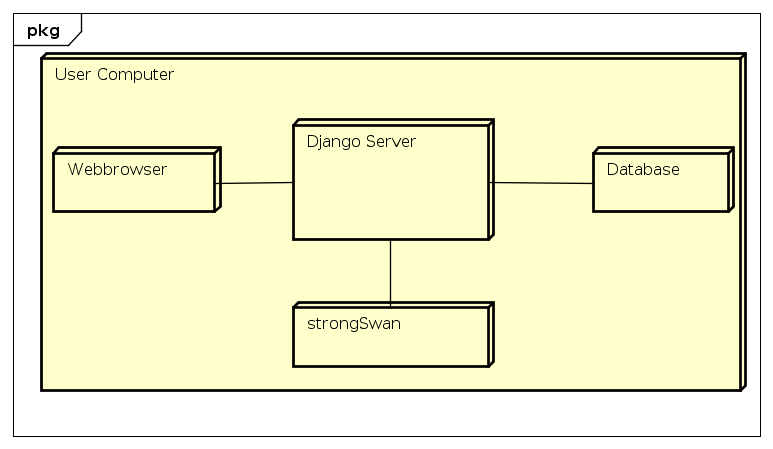
\includegraphics[width=360pt]{images/deployment.png}
\caption[Deployment]{Deployment}
\end{figure}

\subsection{Domain Model}

\begin{figure}[H]
\centering
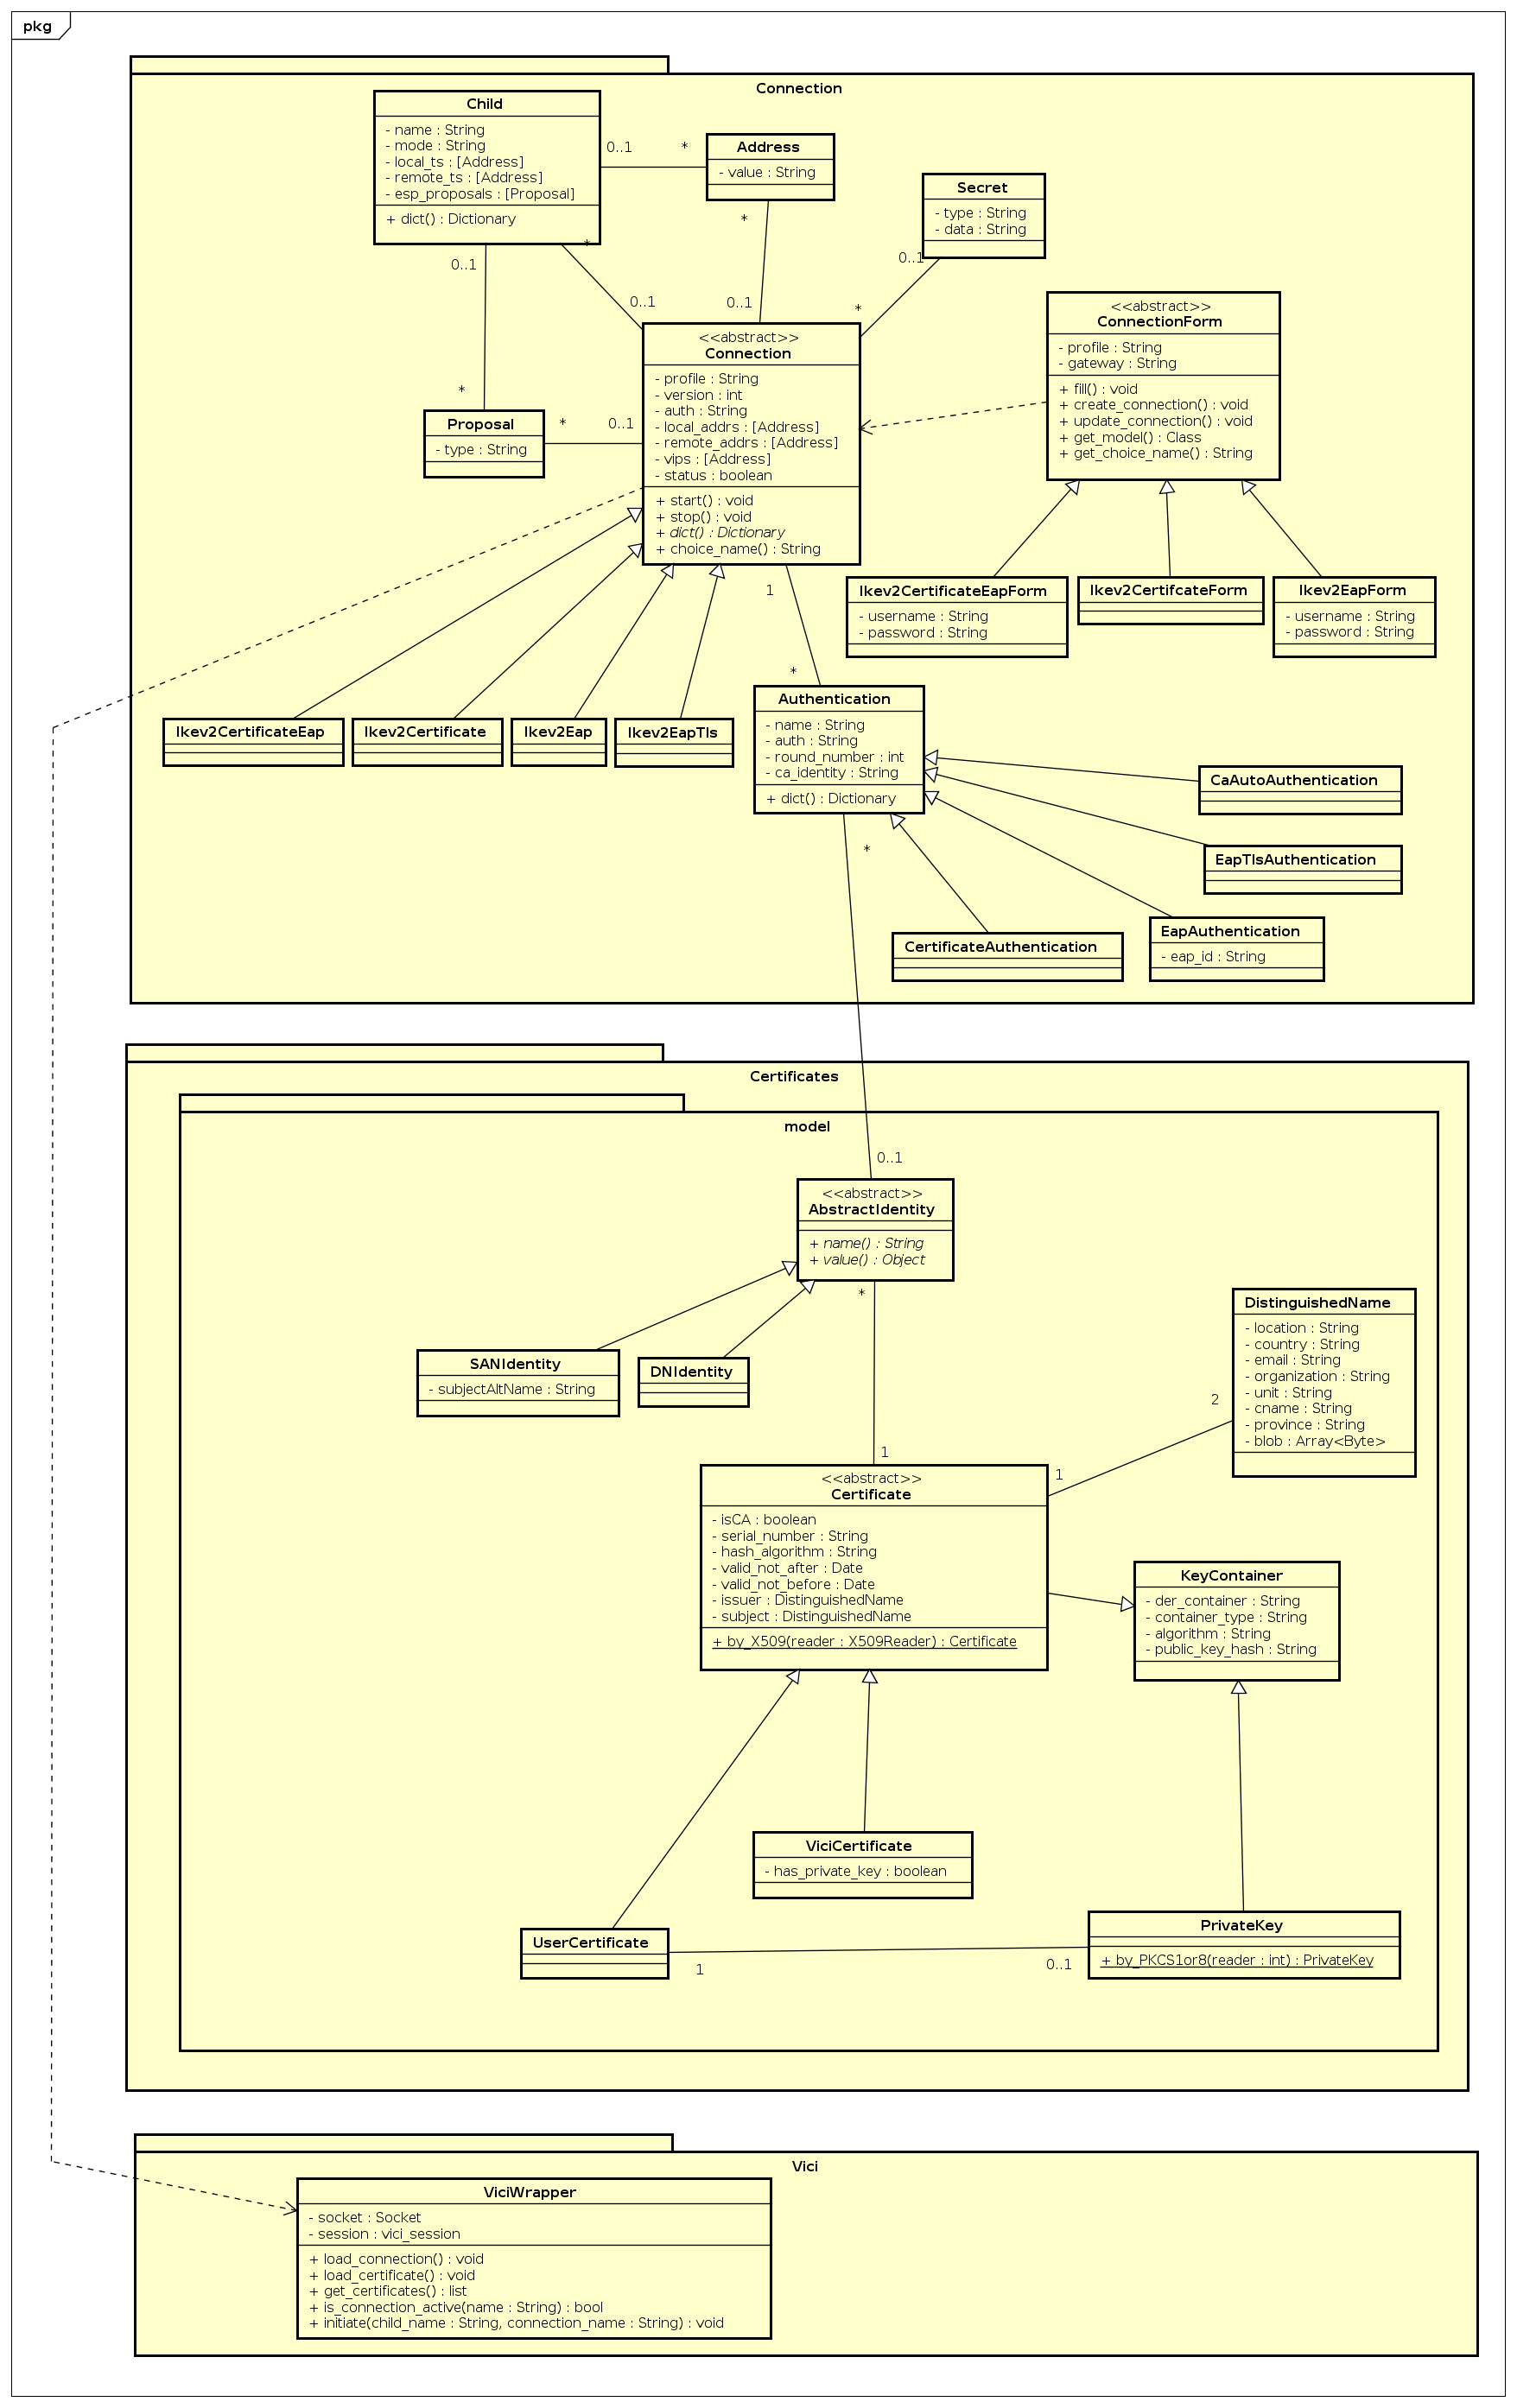
\includegraphics[width=420pt]{images/domain_model_strongman.png}
\caption[Domain Model]{Domain Model}
\end{figure}

Das Domain Model soll im Allgemeinen eine Abstraktion der Vici-Schnittstelle darstellen.
Dabei ist die Connection Klasse zentral. Damit die verschiedenen Authentisierungsmethoden unterstütz werden können, wird von Connection geerbt.

Weiter sind die Certificates ein essentieller Bestandteil, diese sind über die Hilfsklasse AbstractIdentity mit der Authentication verbunden, welche wiederum ein Verbindung zur Connection hat.

\newpage